\section{Foward and Backward pass}
In this section, we will step-by-step brake down every step in a Multi-Layer Neural Network to understand their role in the model as well as figuring the imperative computation of parameters must be accomplised in these steps. 
\begin{figure}[H]
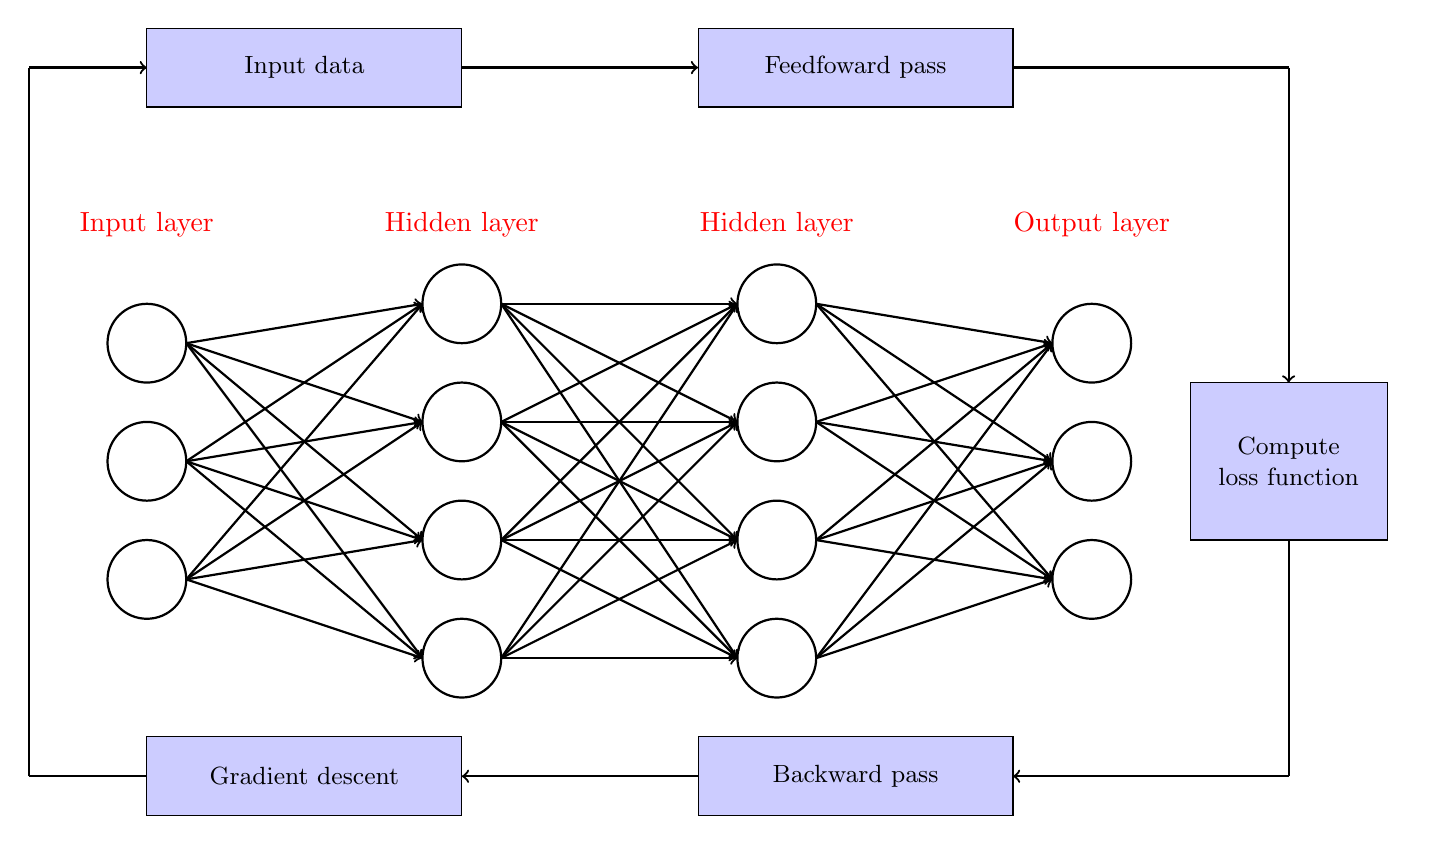
\begin{tikzpicture}


	% neutrons
	\node[red] at (-6,5.5) {Input layer};
	\draw[thick,black] (-6,1) circle (0.5cm);
	\draw[thick,black] (-6,2.5) circle (0.5cm);
	\draw[thick,black] (-6,4) circle (0.5cm);


	\node[red] at (-2,5.5) {Hidden layer};
	\draw[thick,black] (-2,0) circle (0.5cm);
	\draw[thick,black] (-2,1.5) circle (0.5cm);
	\draw[thick,black] (-2,3) circle (0.5cm);
	\draw[thick,black] (-2,4.5) circle (0.5cm);


	\node[red] at (2,5.5) {Hidden layer};
	\draw[thick,black] (2,0) circle (0.5cm);
	\draw[thick,black] (2,1.5) circle (0.5cm);
	\draw[thick,black] (2,3) circle (0.5cm);
	\draw[thick,black] (2,4.5) circle (0.5cm);


	\node[red] at (6,5.5) {Output layer};
	\draw[thick,black] (6,1) circle (0.5cm);
	\draw[thick,black] (6,2.5) circle (0.5cm);
	\draw[thick,black] (6,4) circle (0.5cm);

	% blocks

	\draw[fill=blue!20] (-6,8) rectangle (-2,7); % input block
	\draw[fill=blue!20] (1,8) rectangle (5,7); % feedforward block
	\draw[fill=blue!20] (7.25,3.5) rectangle (9.75,1.5);  % prediction block
	\draw[fill=blue!20] (1,-1) rectangle (5,-2);  % backward block
	\draw[fill=blue!20] (-6,-1) rectangle (-2,-2);  % gradient descend block
	
	% label
	\node[black,font=\small] at (-4,7.5) {Input data};
	\node[black,font=\small] at (3,7.5) {Feedfoward pass};
	\node[black,font=\small,text width=3cm,align=center] at (8.5,2.5) {Compute loss function};
	\node[black,font=\small] at (3,-1.5) {Backward pass};
	\node[black,font=\small] at (-4,-1.5) {Gradient descent};
	%Links
	% arror of process
	\draw[->,thick] (-2,7.5) -- (1,7.5); % link from input data to feedforward pass
	\draw[-,thick] (5,7.5) -- (8.5,7.5); % link from feedforward pass to intermediate point 1
	\draw[->,thick] (8.5,7.5) -- (8.5,3.5); % link from intermediate point 1 to compute loss function
	\draw[-,thick](8.5,1.5) -- (8.5,-1.5); % link from compute loss function to intermediate 2
	\draw[->,thick](8.5,-1.5) -- (5,-1.5); % link from intermediate point 2 to backward pass
	\draw[->,thick] (1,-1.5) -- (-2,-1.5); % link from backward pass to gradient descend
	\draw[-,thick] (-6,-1.5) -- (-7.5,-1.5); % link from gradient descend to intermedidate point 3
	\draw[-,thick] (-7.5,-1.5) -- (-7.5,7.5) ; % to intermedidate point 3 to intermediate point 4
	\draw[->,thick] (-7.5,7.5) -- (-6,7.5); % link from intermeidate point 4 to input data
	% input layer to hidden layer 
	\draw[->,thick] (-5.5,1) -- (-2.5,0);
	\draw[->,thick] (-5.5,1) -- (-2.5,1.5);
	\draw[->,thick] (-5.5,1) -- (-2.5,3);
	\draw[->,thick] (-5.5,1) -- (-2.5,4.5);
	
	\draw[->,thick] (-5.5,2.5) -- (-2.5,0);
	\draw[->,thick] (-5.5,2.5) -- (-2.5,1.5);
	\draw[->,thick] (-5.5,2.5) -- (-2.5,3);
	\draw[->,thick] (-5.5,2.5) -- (-2.5,4.5);

	\draw[->,thick] (-5.5,4) -- (-2.5,0);
	\draw[->,thick] (-5.5,4) -- (-2.5,1.5);
	\draw[->,thick] (-5.5,4) -- (-2.5,3);
	\draw[->,thick] (-5.5,4) -- (-2.5,4.5);

	
	% links hidden layer 1 to hidden layer 2
	\draw[->,thick] (-1.5,0) -- (1.5,0);
	\draw[->,thick] (-1.5,0) -- (1.5,1.5);
	\draw[->,thick] (-1.5,0) -- (1.5,3);
	\draw[->,thick] (-1.5,0) -- (1.5,4.5);
	
	\draw[->,thick] (-1.5,1.5) -- (1.5,0);
	\draw[->,thick] (-1.5,1.5) -- (1.5,1.5);
	\draw[->,thick] (-1.5,1.5) -- (1.5,3);
	\draw[->,thick] (-1.5,1.5) -- (1.5,4.5);

	\draw[->,thick] (-1.5,3) -- (1.5,0);
	\draw[->,thick] (-1.5,3) -- (1.5,1.5);
	\draw[->,thick] (-1.5,3) -- (1.5,3);
	\draw[->,thick] (-1.5,3) -- (1.5,4.5);

	\draw[->,thick] (-1.5,4.5) -- (1.5,0);
	\draw[->,thick] (-1.5,4.5) -- (1.5,1.5);
	\draw[->,thick] (-1.5,4.5) -- (1.5,3);
	\draw[->,thick] (-1.5,4.5) -- (1.5,4.5);


	% links hidden layer 2 to output layer
	\draw[->,thick] (2.5,0) -- (5.5,1);
	\draw[->,thick] (2.5,0) -- (5.5,2.5);
	\draw[->,thick] (2.5,0) -- (5.5,4);
	
	\draw[->,thick] (2.5,1.5) -- (5.5,1);
	\draw[->,thick] (2.5,1.5) -- (5.5,2.5);
	\draw[->,thick] (2.5,1.5) -- (5.5,4);

	\draw[->,thick] (2.5,3) -- (5.5,1);
	\draw[->,thick] (2.5,3) -- (5.5,2.5);
	\draw[->,thick] (2.5,3) -- (5.5,4);

	\draw[->,thick] (2.5,4.5) -- (5.5,1);
	\draw[->,thick] (2.5,4.5) -- (5.5,2.5);
	\draw[->,thick] (2.5,4.5) -- (5.5,4);

\end{tikzpicture}
\caption{Procedure to find the optimal solution in Multi-layer Neural Network}
\centering
\end{figure}
Generally, a basic Multi-layer Neural Network consists of 5 steps:\newline
\begin{itemize}
	\item \textbf{Load input data:} data is fed into the network. Depend on the optimization strategy, the number of data input can be different.
	\item \textbf{Feedforward pass:} calculate the activation output of neurons for all layers based on \textit{non-linear} operation.
	\item \textbf{Compute loss function:} the loss function is computed in the output layer to quantify the performance of the model's optimization.
	\item \textbf{Backward pass:} calculate the gradient of loss function w.r.t the parameters weight matrix $w^{l}$ and bias vector $b^{l}$
	\item \textbf{Gradient descend:} the parameters $w^{l}$,$b^{l}$ are updated by using gradient of cost function to improve the performace. Unless the model completely loads every element in the dataset, the new input unit will be continuously fed into the model.
\end{itemize}
Once the \textbf{Backward pass} is reached, a new data will be fed to feedforward pass again to redo the exact procedure until the model either achieves favoriable performance or fails to solve the problem.

\subsection{Forward Pass}
For the forward pass of neuron network, or so also known as a perceptron, we define the weighted input to a neuron $l^{th}$ by:
\begin{equation}
	z^{l}_{j} = \Sigma_{k} w^{l}_{kj}a^{l-1}_{k} + b^{l}_{j}
\end{equation}
where:\newline
$a^{l-1}_{k}$ is the input from the neuron $k^{th}$ of layer $(l-1)^{th}$\newline
$w^{l}_{kj}$ is the weight corresponding to the link between neuron $k^{th}$ of layer $(l-1)^{th}$ and neuron $j^{th}$ of layer $l^{th}$\newline
$b^{l}_{j}$ is the bias term of the neuron $j^{th}$ of the layer $l^{th}$\newline
\newline
The weighted input to neuron $z^{k}_{j}$ is passed through an activation function $\sigma()$ (which will be carefully declared in chapter 2). The result of activation function will either become the next layer's neurons input or the output of the network. Then we obtain the expectated output of the neuron $j^{th}$ of layer $l^{th}$ as follow:
\begin{equation}\label{eq:neuron_output}
	a^{l}_{j} = \sigma\left(\Sigma_{k} w^{l}_{kj}a^{l-1}_{k} + b^{l}_{j}\right)
\end{equation}
u
In fact, this representation \eqref{eq:neuron_output} only well describe the output of a single neuron. In practice, we would like utilize the power of linear algebra in order to avoid looping so many time to calculate for each neuron in the layer. Because of this, we would like to rewrite the \eqref{eq:neuron_output} in the matrix form:
\begin{equation}\label{eq:neuron_output_matrix_form}
	a^{l} = \sigma\left(w^{l}a^{l-1} + b^{l}\right)
\end{equation}
\textbf{Remark 1:}the activation function for \eqref{eq:neuron_output_matrix_form} is \textbf{element-wise} function.\newline\noindent
\textbf{Remark 2:}some textbooks may write \eqref{eq:neuron_output_matrix_form} as $a^{l} = \sigma\left((w^{l})^{T}a^{l-1} + b^{l}\right)$ in which the weight matrix $w^{l}$ is transposed.This unsynchronization is dued to the difference in notation of the weight matrix component $w^{l}_{jk}$ in \eqref{eq:neuron_output} where we use the inverse order of relationship between 2 connected neurons, e.g the ``suppose'' to be correct description for this parameter is ``the weight between neuron $k^{th}$-layer $(l-1)^{th}$ connects to neuron $j^{th}$-layer $l^{th}$'', so the precise notation should have been \textbf{$w^{l}_{kj}$}. But once we use the reverse notation, it allows us to get rid of the transpose operation for matrix representation!

\begin{figure}[H]
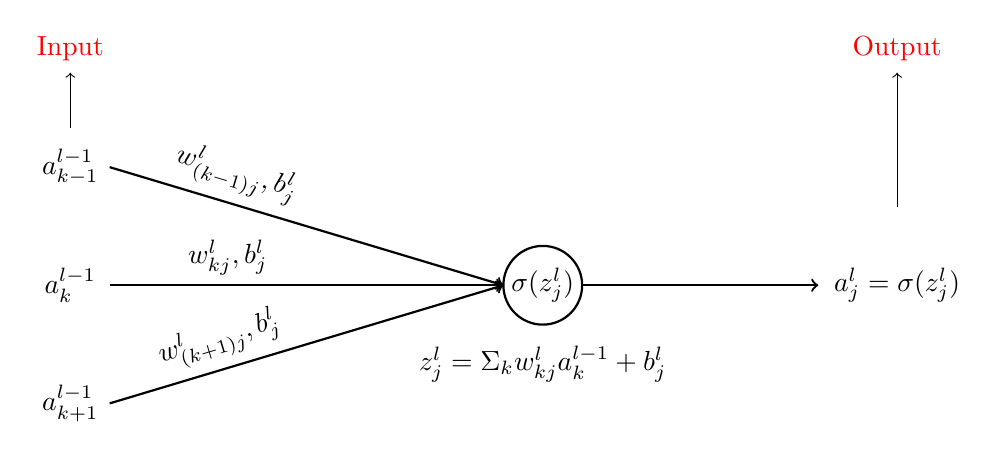
\begin{tikzpicture}  
	
	% Node
	\draw[thick,black] (0,0) circle (0.5cm);
	\node[black] at (0,0) {$\sigma(z^{l}_{j})$};
	\node[black] at (0,-1) {$z^{l}_{j}=\Sigma_{k}w^{l}_{kj}a^{l-1}_{k} + b^{l}_{j}$};
	\node[black] at (-6,1.5) {$a^{l-1}_{k-1}$};
	\node[black] at (-6,0) {$a^{l-1}_{k}$};
	\node[black] at (-6,-1.5) {$a^{l-1}_{k+1}$};
	\node[black] at (4.5,0) {$a^{l}_{j}=\sigma(z^{l}_{j})$};
	
	%Label
	\node[red] at (-6,3) {Input};
	\node[red] at (4.5,3) {Output};

	
	%link
	\draw[->,thick] (-5.5,1.5) -- (-0.5,0) node[pos=0.3,above,sloped] {$w^{l}_{(k-1)j},b^{l}_{j}$};
	\draw[->,thick] (-5.5,0) -- (-0.5,0) node[pos=0.3,above] {$w^{l}_{kj},b^{l}_{j}$};
	\draw[->,thick] (-5.5,-1.5) -- (-0.5,0) node[pos=0.3,above,sloped] {$w^{l}_{(k+1)j},b^{l}_{j}$};
	\draw[->,thick] (0.5,0) -- (3.5,0) node[midway,above] {}; 
	\draw[->,thin] (-6,2) -- (-6,2.7) ;
	\draw[->,thin] (4.5,1) -- (4.5,2.7) ;

\end{tikzpicture}
\centering
	\caption{Illustration input and output of a neuron}
\end{figure}

\subsection{Backward pass (Backpropagation)}
\textbf{Objective:} calculate the rate of change of loss function w.r.t the weight and the bias of each layer. Unfortunately, we don't have direct formulas to accomplish this job, but we can still calculate these unknowns through 2 supporting equations that will be derived as follow.
\vspace{0.5cm}\newline\noindent
\textit{Calculating the error in the output layer}\newline \noindent
\begin{figure}[H]
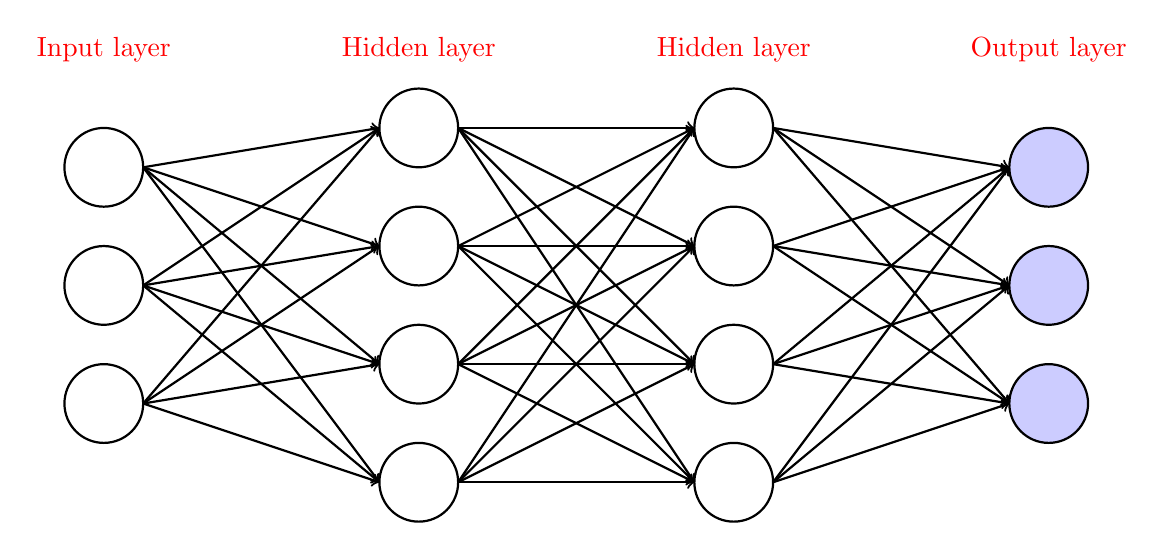
\begin{tikzpicture}
% neutrons
	\node[red] at (-6,5.5) {Input layer};
	\draw[thick,black] (-6,1) circle (0.5cm);
	\draw[thick,black] (-6,2.5) circle (0.5cm);
	\draw[thick,black] (-6,4) circle (0.5cm);


	\node[red] at (-2,5.5) {Hidden layer};
	\draw[thick,black] (-2,0) circle (0.5cm);
	\draw[thick,black] (-2,1.5) circle (0.5cm);
	\draw[thick,black] (-2,3) circle (0.5cm);
	\draw[thick,black] (-2,4.5) circle (0.5cm);


	\node[red] at (2,5.5) {Hidden layer};
	\draw[thick,black] (2,0) circle (0.5cm);
	\draw[thick,black] (2,1.5) circle (0.5cm);
	\draw[thick,black] (2,3) circle (0.5cm);
	\draw[thick,black] (2,4.5) circle (0.5cm);


	\node[red] at (6,5.5) {Output layer};
	\draw[draw=black,thick,,fill=blue!20] (6,1) circle (0.5cm);
	\draw[draw=black,thick,fill=blue!20] (6,2.5) circle (0.5cm);
	\draw[draw=black,thick,fill=blue!20] (6,4) circle (0.5cm);

	%Links
	% input layer to hidden layer 
	\draw[->,thick] (-5.5,1) -- (-2.5,0);
	\draw[->,thick] (-5.5,1) -- (-2.5,1.5);
	\draw[->,thick] (-5.5,1) -- (-2.5,3);
	\draw[->,thick] (-5.5,1) -- (-2.5,4.5);
	
	\draw[->,thick] (-5.5,2.5) -- (-2.5,0);
	\draw[->,thick] (-5.5,2.5) -- (-2.5,1.5);
	\draw[->,thick] (-5.5,2.5) -- (-2.5,3);
	\draw[->,thick] (-5.5,2.5) -- (-2.5,4.5);

	\draw[->,thick] (-5.5,4) -- (-2.5,0);
	\draw[->,thick] (-5.5,4) -- (-2.5,1.5);
	\draw[->,thick] (-5.5,4) -- (-2.5,3);
	\draw[->,thick] (-5.5,4) -- (-2.5,4.5);

	
	% hidden layer 1 to hidden layer 2
	\draw[->,thick] (-1.5,0) -- (1.5,0);
	\draw[->,thick] (-1.5,0) -- (1.5,1.5);
	\draw[->,thick] (-1.5,0) -- (1.5,3);
	\draw[->,thick] (-1.5,0) -- (1.5,4.5);
	
	\draw[->,thick] (-1.5,1.5) -- (1.5,0);
	\draw[->,thick] (-1.5,1.5) -- (1.5,1.5);
	\draw[->,thick] (-1.5,1.5) -- (1.5,3);
	\draw[->,thick] (-1.5,1.5) -- (1.5,4.5);

	\draw[->,thick] (-1.5,3) -- (1.5,0);
	\draw[->,thick] (-1.5,3) -- (1.5,1.5);
	\draw[->,thick] (-1.5,3) -- (1.5,3);
	\draw[->,thick] (-1.5,3) -- (1.5,4.5);

	\draw[->,thick] (-1.5,4.5) -- (1.5,0);
	\draw[->,thick] (-1.5,4.5) -- (1.5,1.5);
	\draw[->,thick] (-1.5,4.5) -- (1.5,3);
	\draw[->,thick] (-1.5,4.5) -- (1.5,4.5);


	% hidden layer 2 to output layer
	\draw[->,thick] (2.5,0) -- (5.5,1);
	\draw[->,thick] (2.5,0) -- (5.5,2.5);
	\draw[->,thick] (2.5,0) -- (5.5,4);
	
	\draw[->,thick] (2.5,1.5) -- (5.5,1);
	\draw[->,thick] (2.5,1.5) -- (5.5,2.5);
	\draw[->,thick] (2.5,1.5) -- (5.5,4);

	\draw[->,thick] (2.5,3) -- (5.5,1);
	\draw[->,thick] (2.5,3) -- (5.5,2.5);
	\draw[->,thick] (2.5,3) -- (5.5,4);

	\draw[->,thick] (2.5,4.5) -- (5.5,1);
	\draw[->,thick] (2.5,4.5) -- (5.5,2.5);
	\draw[->,thick] (2.5,4.5) -- (5.5,4);
\end{tikzpicture}
\centering
\caption{Calculating the error of output layer}
\end{figure}

The error of neuron \textit{$j^{th}$} of the output layer \textit{L} is calculated by
\begin{equation}
    \delta^{L}_{j} = \frac{\partial \mathcal{C}}{\partial a^{L}_{j}} \sigma^{'}(z^{L}_{j})
\end{equation}
or in matrix form:
\begin{equation}\label{eq:erroroutput}
    \delta^{L} = \nabla_{a} \mathcal{C}\odot \sigma^{'}(z^{L})
\end{equation}
where $\frac{\partial \mathcal{C}}{\partial a^{L}_{j}}$ indicates how fast the cost function changes w.r.t the output layer activation of neuron \textit{$j^{th}$}
and $\sigma^{'}(z^{L}_{j})$ measures the rate of change of activation function $\sigma$ w.r.t the $z^{L}_{j}$. In the matrix form, $\odot$ is called Hadamard product. The result of $u \odot v$ is the element-wise product $u_{i}$ and $v_{i}$ of $u$ and $v$ respectively. Moreover, $\nabla$ is called ``nabla'' - the notation for vector differential operation.\newline
\newline\noindent
\textbf{Interpretation:} this factor allows us to know the dependency of the cost function $C$ on the output neuron $j^{th}$. If the neuron $j^{th}$ of the output layer doesn't contribute much to the cost function result, then the error $\delta^{L}$ should be small\newline
\newline
For example: $\mathcal{C}$ is MSE function $\mathcal{C} = || a^{L} - y||_{2}$ then the error $\delta^{L}$ is calculated by: $\delta^{L} = (a^{L} - y) \odot \sigma^{'}(z^{L})$\newline

\vspace{1.5cm}\noindent
\textit{Calculate the error $\delta^{l}$ in terms of the error in the next layer $\delta^{l+1}$}
\begin{equation}
	\delta^{l}_{k} = (w^{l+1}_{jk}) (\delta^{l+1}_{j})  \sigma^{'}(z^{l}_{k})
\end{equation}
or in matrix form:
\begin{equation} \label{eq:errorhidden}
	\delta^{l} = ((w^{l+1})^{T} \delta^{l+1}) \odot \sigma^{'}(z^{l})
\end{equation}
\begin{figure}[H] 
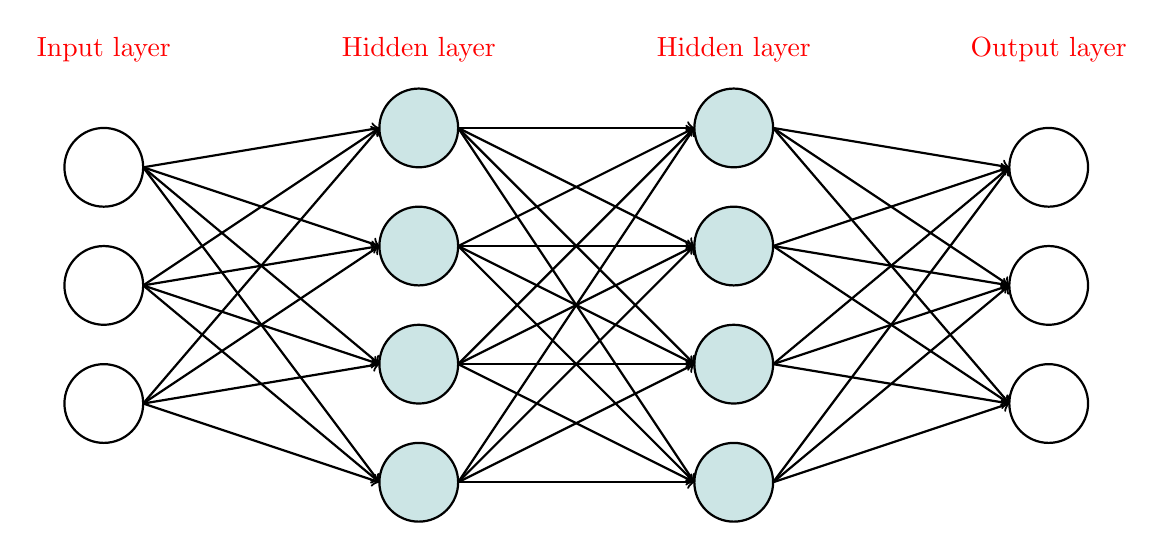
\begin{tikzpicture}
% neutrons
	\node[red] at (-6,5.5) {Input layer};
	\draw[thick,black] (-6,1) circle (0.5cm);
	\draw[thick,black] (-6,2.5) circle (0.5cm);
	\draw[thick,black] (-6,4) circle (0.5cm);


	\node[red] at (-2,5.5) {Hidden layer};
	\draw[thick,black,fill=teal!20] (-2,0) circle (0.5cm);
	\draw[thick,black,fill=teal!20] (-2,1.5) circle (0.5cm);
	\draw[thick,black,fill=teal!20] (-2,3) circle (0.5cm);
	\draw[thick,black,fill=teal!20] (-2,4.5) circle (0.5cm);


	\node[red] at (2,5.5) {Hidden layer};
	\draw[thick,black,fill=teal!20] (2,0) circle (0.5cm);
	\draw[thick,black,fill=teal!20] (2,1.5) circle (0.5cm);
	\draw[thick,black,fill=teal!20] (2,3) circle (0.5cm);
	\draw[thick,black,fill=teal!20] (2,4.5) circle (0.5cm);


	\node[red] at (6,5.5) {Output layer};
	\draw[draw=black,thick] (6,1) circle (0.5cm);
	\draw[draw=black,thick] (6,2.5) circle (0.5cm);
	\draw[draw=black,thick] (6,4) circle (0.5cm);

	%Links
	% input layer to hidden layer 
	\draw[->,thick] (-5.5,1) -- (-2.5,0);
	\draw[->,thick] (-5.5,1) -- (-2.5,1.5);
	\draw[->,thick] (-5.5,1) -- (-2.5,3);
	\draw[->,thick] (-5.5,1) -- (-2.5,4.5);
	
	\draw[->,thick] (-5.5,2.5) -- (-2.5,0);
	\draw[->,thick] (-5.5,2.5) -- (-2.5,1.5);
	\draw[->,thick] (-5.5,2.5) -- (-2.5,3);
	\draw[->,thick] (-5.5,2.5) -- (-2.5,4.5);

	\draw[->,thick] (-5.5,4) -- (-2.5,0);
	\draw[->,thick] (-5.5,4) -- (-2.5,1.5);
	\draw[->,thick] (-5.5,4) -- (-2.5,3);
	\draw[->,thick] (-5.5,4) -- (-2.5,4.5);

	
	% hidden layer 1 to hidden layer 2
	\draw[->,thick] (-1.5,0) -- (1.5,0);
	\draw[->,thick] (-1.5,0) -- (1.5,1.5);
	\draw[->,thick] (-1.5,0) -- (1.5,3);
	\draw[->,thick] (-1.5,0) -- (1.5,4.5);
	
	\draw[->,thick] (-1.5,1.5) -- (1.5,0);
	\draw[->,thick] (-1.5,1.5) -- (1.5,1.5);
	\draw[->,thick] (-1.5,1.5) -- (1.5,3);
	\draw[->,thick] (-1.5,1.5) -- (1.5,4.5);

	\draw[->,thick] (-1.5,3) -- (1.5,0);
	\draw[->,thick] (-1.5,3) -- (1.5,1.5);
	\draw[->,thick] (-1.5,3) -- (1.5,3);
	\draw[->,thick] (-1.5,3) -- (1.5,4.5);

	\draw[->,thick] (-1.5,4.5) -- (1.5,0);
	\draw[->,thick] (-1.5,4.5) -- (1.5,1.5);
	\draw[->,thick] (-1.5,4.5) -- (1.5,3);
	\draw[->,thick] (-1.5,4.5) -- (1.5,4.5);


	% hidden layer 2 to output layer
	\draw[->,thick] (2.5,0) -- (5.5,1);
	\draw[->,thick] (2.5,0) -- (5.5,2.5);
	\draw[->,thick] (2.5,0) -- (5.5,4);
	
	\draw[->,thick] (2.5,1.5) -- (5.5,1);
	\draw[->,thick] (2.5,1.5) -- (5.5,2.5);
	\draw[->,thick] (2.5,1.5) -- (5.5,4);

	\draw[->,thick] (2.5,3) -- (5.5,1);
	\draw[->,thick] (2.5,3) -- (5.5,2.5);
	\draw[->,thick] (2.5,3) -- (5.5,4);

	\draw[->,thick] (2.5,4.5) -- (5.5,1);
	\draw[->,thick] (2.5,4.5) -- (5.5,2.5);
	\draw[->,thick] (2.5,4.5) -- (5.5,4);
\end{tikzpicture}
\centering
\caption{Calculating the error of hidden layers}
\label{fig:errorlayer}
\end{figure}
where $\delta^{l+1}$,$w^{l+1}$ are the error and weight terms of the next layer or the right next layer according to the figure~\ref{fig:errorlayer}\newline \noindent
\textbf{Interpretation:} initially once we compute the~\eqref{eq:errorhidden}, we then have enough ``inertia' to go backward from the output layer back to input layer direction in order to calculate the error term for each hidden layer.

\vspace{0.2cm} \noindent
Now with the support from \eqref{eq:erroroutput} and~\eqref{eq:errorhidden}, we are confident to say that the goal of backpropagation is feasible to achieve. The formulas to estimate the rate of change of the loss function $C$ w.r.t the weight and bias of each layer are:\newline \noindent
\newline \noindent
\textit{Calculate the rate of change of the cost w.r.t any bias in the network}
\begin{equation}\label{eq:errorbias}
    \frac{\partial \mathcal{C}}{\partial b^{l}_{j}} = \delta^{l}_{j}
\end{equation}
The equation is straightforward! The rate of change of loss fucntion w.r.t the bias is \underline{\smash{the error of each layer}}.

\vspace{1.5cm}\noindent
\textit{Calculate the rate of change of the cost w.r.t any weight in the network}
\begin{equation}%\label{eq:errorweight}
    \frac{\partial \mathcal{C}}{\partial w^{l}_{jk}} = a^{l-1}_{k} \delta^{l}_{j} \label{eq:errorweight}
\end{equation}
the rate of change of the cost w.r.t the weight is depended on the activation output of neuron $k^{th}$ of layer $(l-1)^{th}$ and the error term of neuron $l^{th}$ of layer $l^{th}$ itself.\newline\noindent
\newline\noindent
\textbf{Evaluation: What can we perceive from the result of \eqref{eq:errorbias} and \eqref{eq:errorweight}?}\newline\noindent
\textbf{Answer:} the $\frac{\partial C}{\partial w}$ is \underline{\smash{small}} meaning that the weight tend to update their weight \underline{\smash{slower}}. There are factors that can cause this result: (1) when the activation ouput $a^{l-1}_{k} \approx 0$, (2) when the error $\delta^{l}_{j} \approx 0$\newline \noindent
For $1^{th}$ factor to the design of activation function that can force the weight input to low value.\newline\noindent
For $2^{th}$ factor we must go backward to the error of output layer at \eqref{eq:erroroutput}. When the rate of change of activation of output layer $\sigma^{'}(z^{L}_{j})$ is small, it means that the output neuron had stepped to saturated region where $z^{L}_{J}$ is not likely to vary its value. Then the error of output neuron $j^{th}$ is small and makes the error term $\delta^{l}_{k}$ is small as well according to \eqref{eq:errorhidden}.\newline \noindent
The explaination for the bias gradient hold the same idea as above. The phenomenom when gradient of weight $\frac{\partial \mathcal{C}}{w}$ and gradient of bias $\frac{\partial \mathcal{C}}{b}$ are becoming very small \underline{\smash{during the training}} (when the loss function is not yet minimized) is called \textbf{vanishing gradient}. The original source of such phenomenom is from the degradation of activation gradient $\sigma^{'}(z^{l})$ which triggers a chain effect to $\frac{\partial \mathcal{C}}{b}$,$\frac{\partial \mathcal{C}}{w}$. Depend on the usage of activation function, we are going to analyze clearer the way to get rid of vanishing gradient in section 3\newline\noindent
\newline\noindent
\section{Optimizer}
\subsection{Gradient Descent and its variants}

\subsubsection{Stochastic Gradient Descent (SGD)}
This is the most naive way to update the weight matrix as this optimizer repeats the update sequentially for every 1 input sample.  
\textit{Weight update formula for any layer in SGD}
\begin{equation}
    w^{l} := w^{l} - \alpha \nabla_{w^{l}} \mathcal{C}
\end{equation}
where $\alpha > 0$ is the learning rate
\subsubsection{Batch Gradient Descent}
Instead of considering 1 input only, the idea of batch GD is to feed the entire dataset to the neural network. What is changed in batch GD formula compares to SGD formula is the update subtrahende term as it becomes the average of all subtrahends corresponding to each data sample. We adjust batch formula based on the computation of the loss function for the whole dataset with A samples:
\begin{equation}
    \mathcal{C}_{w} = \frac{1}{N} \sum^{A}_{i=1} \mathcal{C}_{w}(x_{i},y_{i})
\end{equation}
Then the batch GD becomes:
\begin{equation}
    w^{l} := w^{l} - \alpha \frac{1}{A} \sum^{N}_{i=1} \nabla_{w^{l}} \mathcal{C}(x_{i},y_{i})
\end{equation}
Remind that we will implement vectorization for these formula, so if the dataset has A samples, then the dimension of $\nabla_{w^{l}}C$ matrix is (A,N,M) but the dimension of $w^{l}$ is still (N,M) (N,M are the height and width of weight matrix of each layer).\newline\noindent
One reason that batch GD is not so commonly used is because the size of dataset is usually very large nowadays such that it is no longer economical to upgrade the hardware for loading the entire dataset. Moreover, the efficiency of this optimizer is not always assured since the weight matrix is updated only 1 time which may not bring the best converged result for the model.

\subsubsection{Mini-Batch Gradient Descent}
Mini-Batch has the same idea as batch GD except the fact this strategy split the dataset into many batchs and feed them to the model one-by-one. That means, the weight will be updated more frequently and still be able to ultize the parallelization computational power of the hardware. Given a dataset that is split into B batchs, each with C samples, then the formula to update the weight for 1 batch is:
\begin{equation}
    w^{l} := w^{l} - \alpha \frac{1}{A} \sum^{C}_{i=1} \nabla_{w^{l}} \mathcal{C}(x_{i},y_{i})
\end{equation}
Mini-batch is one of the widely used strategy for optimization the neural network.
\subsubsection{Stochastic Gradient Descent with Momentum}
The SGD with momentum offers a velocity terms to speed up the optimizating step, especially when the neural network model get stuck at a local minimum. In that case, if the \textit{learning rate} is set small, the model will accept the local minimum as general solution hence unable to optimize the model. On the contrary, if we would like to get rid of this aannoying issue by simply setting the \textit{learning rate} to a bigger value, then probally we can accidentally ``jump'' over the global minimum. These problems are indicated in figure \ref{fig:issueLR}.

\begin{figure}[h]
    \fbox{
    \begin{tikzpicture}
        \draw[thick] (-1,8) 
        .. controls (2.5,-0.8) .. (5,6) % global minimum (2.5,-0.8)
        .. controls (5.7,8) and (11,1)..(13, 12); %local minimum (11,1) 

        % global minimum
        \draw[thin] (2.5,1.1) circle (0.2cm);
        \fill[green!70](2.5,1.1) circle (0.2cm);
        \node at (2.5,0.5) {\small{Global minimum}};
        % approximate solution
        \draw[thin] (3.4,2) circle (0.2cm);
        \fill[red!70](3.4,2) circle (0.2cm);
        
        \draw[thin] (1.3,2.5) circle (0.2cm);
        \fill[red!70](1.3,2.5) circle (0.2cm);

        \draw[thin] (3.6,2.6) circle (0.2cm);
        \fill[red!70](3.6,2.6) circle (0.2cm);
        
        \draw[thin] (1.7,2) circle (0.2cm);
        \fill[red!70](1.7,2) circle (0.2cm);
        
        \draw[->,thin] (3.2,2) -- (1.5,2.5);
        \draw[->,thin] (1.5,2.5) -- (3.4,2.6);
        \draw[->,thin] (3.4,2.6) -- (1.9,2);
        % local minum
        \draw[thin] (9,5.6) circle (0.2cm);
        \fill[red!70](9,5.6) circle (0.2cm);
        
        \draw[thin] (8.8,5.6) circle (0.2cm);
        \fill[red!70](8.8,5.6) circle (0.2cm);
        
        \draw[thin] (8.6,5.6) circle (0.2cm);
        \fill[red!70](8.6,5.6) circle (0.2cm);
        
        \draw[thin] (8.4,5.6) circle (0.2cm);
        \fill[red!70](8.4,5.6) circle (0.2cm);
        \node at (9,7) {\small{Local minimum}};

        % arrow
        \draw[->,thick] (8.5,6) -- (7,6.4);
    \end{tikzpicture}}
    \centering
    \caption{Illustration for big \textit{learning rate} and small \textit{learning rate}  situation. In the former case, the red points are the attemps of neural network model to approach optimized point (green point) but large LR occurs the next update value keep jumpng around the global bottom point. In the later case, we can see multiple attemps to pass the local maxima but because of small LR, the updated effort is very slow.}
    \label{fig:issueLR}
\end{figure}

Hence a new variable $v$ which defines the velocity (speed and direction) for the gradient descent algorithm upgrading purpose. The SGD with momentum algorithm now contains 2 formulas; Given a dataset that is split into B batchs, each with C samples, then the formula to update the weight for 1 batch is:
\begin{equation}
    \begin{aligned}
        v &= \alpha v - \epsilon \nabla_{\theta} \left( \frac{1}{A} \sum^{C}_{i=1} \nabla_{w^{l}} \mathcal{C}(x_{i},y_{i}) \right) \\
        w^{l} &= w^{l} + v\\
    \end{aligned}
\end{equation}
where $\alpha \in \left[0,1\right)$ is hyperparameter which controls the rate of previous velocity.
\subsection{Nesterov Accelerated Gradient}
Given a dataset that is split into B batchs, each with C samples, then the formula to update the weight for 1 batch is:
\begin{equation}
    \begin{aligned}
        v &= \alpha v - \epsilon \nabla_{\theta} \left( \frac{1}{A} \sum^{C}_{i=1} \mathcal{C}(f(x_{i};w^{l} + \alpha v),y_{i}) \right) \\
        w^{l} &= w^{l} + v\\
    \end{aligned}
\end{equation}
\subsection{Adaptive Gradient Algorithm (Adagrad)}

\subsection{Root Mean Square Propagation (RMSProp)}

\subsection{Adaptive Moment Estimation (Adam) and its variants}

\subsubsection{Adaptive Moment Estimation (Adam)}

\subsubsection{Adam with Weight Decay (AdamW)}

\subsubsection{AdamMax}

\subsubsection{Nesterov-accelerated Adam (Nadam)}


\section{Activation function} 

\subsection{Sigmoid function}
\begin{equation}
    f(x) = \frac{1}{1 + e^{-x}}
\end{equation}

\begin{figure}[H]
    \fbox{
\begin{tikzpicture}
    \begin{axis}[
        domain=-6:6,            % Range of x-values
        samples=100,            % Number of samples for smooth curve
        axis lines=middle,      % Draw axes in the middle
        xlabel={$x$},           % Label for x-axis
        ylabel={$f(x)$},        % Label for y-axis
        ymin=0, ymax=1,         % Range of y-values
        enlargelimits=true,     % Add some space around the plot
        tick label style={font=\small}, % Adjust font size of tick labels
        every axis y label/.style={at={(ticklabel* cs:1)}, anchor=south}, % Adjust y label position
        every axis x label/.style={at={(ticklabel* cs:1)}, anchor=west},  % Adjust x label position
        %grid=both,              % Add grid lines
    ]
        % Plot the sigmoid function
        \addplot[blue, thick] {\sigmoid};
    \end{axis}
\end{tikzpicture}
    }
    \centering
    \caption{Sigmoid function}
\end{figure}

\subsection{Softmax function}
\begin{equation}
    f(x_{i}) = \frac{e^{x_{i}}}{\sum_{j}e^{j}}
\end{equation}

\begin{figure}[H]
    \fbox{
\begin{tikzpicture}
    \begin{axis}[
        domain=-5:5,           % Range of x-values for input
        samples=100,           % Smooth curve
        axis lines=middle,     % Axes in the middle
        xlabel={$x$},          % x-axis label
        ylabel={$f(x)$},          % x-axis label
        ymin=0, ymax=1,        % Range of y-values
        legend style={at={(0.5,-0.15)}, anchor=north, legend columns=-1}, % Legend positioning
        tick label style={font=\small},
        %grid=both,             % Grid lines for readability
    ]

        % Define softmax components for each x_i
        \addplot[blue, thick] {exp(x) / (exp(x) + exp(0) + exp(-2))};

    \end{axis}
\end{tikzpicture}
    }
\centering
    \caption{Softmax function}
\end{figure}

\subsection{Hyperbolic Tangent (Tanh) function}
\begin{equation}
    f(x) = \frac{e^{x} - e^{-x}}{e^{x} + e^{-x}}
\end{equation}
\begin{figure}[H]
    \fbox{
    \begin{tikzpicture}
        \begin{axis}[
            domain=-5:5,           % Range of x-values
            samples=100,           % Smooth curve
            axis lines=middle,     % Axes in the middle
            xlabel={$x$},          % x-axis label
            ylabel={$f(x)$}, % y-axis label
            ymin=-1.2, ymax=1.2,   % Range of y-values
            enlargelimits=true,    % Add some space around the plot
            tick label style={font=\small},
        ]

        % Plot the tanh function
        \addplot[blue, thick] {tanh(x)};
        
    \end{axis}
\end{tikzpicture}
    }
    \centering
    \caption{TanH function}
\end{figure}
\subsection{Rectifier Unit (ReLU) function}
\begin{equation}
    f(x) = \begin{cases}
        x & \text{if x } \geq 0, \\
            0 & \text{if x } < 0
            \end{cases}
\end{equation}
\begin{figure}[H]
    \fbox{
\begin{tikzpicture}
    \begin{axis}[
        domain=-2:4,           % Range of x-values
        samples=100,           % Number of samples for smooth plot
        axis lines=middle,     % Draw axes in the middle
        xlabel={$x$},          % Label for x-axis
        ylabel={$f(x)$},       % Label for y-axis
        ymin=-0.5, ymax=4,     % Range of y-values
        enlargelimits=true,    % Add some space around the plot
        tick label style={font=\small}, % Adjust font size of tick labels
        every axis y label/.style={at={(ticklabel* cs:1)}, anchor=south}, % Adjust y label position
        every axis x label/.style={at={(ticklabel* cs:1)}, anchor=west},  % Adjust x label position
    ]
        % Plot the ReLU function
        \addplot[blue, thick, domain=-2:0] {0};  % Plot y=0 for x < 0
        \addplot[blue, thick, domain=0:4] {x};   % Plot y=x for x >= 0
    \end{axis}
\end{tikzpicture}
    }
    \centering
    \caption{ReLU function}
\end{figure}

\subsection{Leaky Rectifier Unit (LeakyReLU) function}
\begin{equation}
    f(x) = \begin{cases}
        x & \text{if x } \geq 0, \\
            \alpha x & \text{if x } < 0
            \end{cases}
\end{equation}
where $\alpha > 0$

\begin{figure}[H]
    \fbox{
     \begin{tikzpicture}
    \begin{axis}[
        domain=-2:2,           % Range of x-values for input
        samples=100,           % Smooth curve
        axis lines=middle,     % Draw axes in the middle
        xlabel={$x$},          % x-axis label
        ylabel={$f(x)$},       % y-axis label
        ymin=-0.5, ymax=2,     % Range of y-values
        enlargelimits=true,    % Add some space around the plot
        tick label style={font=\small},
    ]

        % Define alpha for Leaky ReLU
        \addplot[blue, thick] {x >= 0 ? x : 0.24*x};
        
    \end{axis}
\end{tikzpicture}  
    }
    \centering 
    \caption{Leaky ReLU function}
\end{figure}
\subsection{Exponential Linear Unit (ELU) function}
\begin{equation}
    f(x) = \begin{cases}
        x & \text{if x} \geq 0 \\
        \alpha(e^{x}-1)& \text{if x } < 0
    \end{cases}
\end{equation}

\begin{figure}[H]
    \fbox{
\begin{tikzpicture}
    \begin{axis}[
        domain=-2:2,           % Range of x-values
        samples=100,           % Smooth curve
        axis lines=middle,     % Axes in the middle
        xlabel={$x$},          % x-axis label
        ylabel={$f(x)$}, % y-axis label
        ymin=-1.5, ymax=2,     % Range of y-values
        enlargelimits=true,    % Add some space around the plot
        tick label style={font=\small},
    ]

        % Define ELU with alpha = 1
        \addplot[blue, thick] {x >= 0 ? x : 0.5*(exp(x) - 1)};
        
    \end{axis}
\end{tikzpicture}
    }
\centering
    \caption{ELU function}
\end{figure}
\subsection{Gaussian Error Linear Unit (GELU) function}
\begin{equation}
    \begin{aligned}
    f(x) =& x\Phi(x) \\
         =& \frac{x}{2} \left(1 + erf\left(\frac{x}{\sqrt{2}}\right) \right)
    \end{aligned}
\end{equation}
where $erf()$ function is

\begin{figure}[H]
    \fbox{
        \begin{tikzpicture}
        \begin{axis}[
            domain=-3:3,           % Range of x-values
            samples=100,           % Smooth curve
            axis lines=middle,     % Axes in the middle
            xlabel={$x$},          % x-axis label
            ylabel={$f(x)$}, % y-axis label
            ymin=-1.5, ymax=3,     % Range of y-values
            enlargelimits=true,    % Add some space around the plot
            tick label style={font=\small},
        ]

        % Plot the GELU function using the approximation formula
        \addplot[blue, thick] {0.5 * x * (1 + tanh(sqrt(2/pi) * (x + 0.044715 * x^3)))};
        
        \end{axis}
        \end{tikzpicture}
    }
    \centering
    \caption{GELU function}
\end{figure}
\subsection{Swish function}
\begin{equation}
    \begin{aligned}
    f(x) =& x \sigma(\beta x) \\
         =& \frac{x}{1+ e^{-\beta x}}
    \end{aligned}
\end{equation}
where $\sigma()$ function is \textit{sigmoid} function

\begin{figure}[H]
    \fbox{
        \begin{tikzpicture}
        \begin{axis}[
            domain=-3:3,           % Range of x-values
            samples=100,           % Smooth curve
            axis lines=middle,     % Axes in the middle
            xlabel={$x$},          % x-axis label
            ylabel={$f(x)$}, % y-axis label
            ymin=-1.5, ymax=3,     % Range of y-values
            enlargelimits=true,    % Add some space around the plot
            tick label style={font=\small},
        ]

        % Plot the GELU function using the approximation formula
        \addplot[blue, thick] {x / (1 + exp(-x))};
        
        \end{axis}
        \end{tikzpicture}
    }
    \centering
    \caption{GELU function}
\end{figure}
\subsection{Maxout function}
\begin{equation}
    f(x) = MAX(w^{T}_{1}x + b_{1},w^{T}_{2}x + b_{2},\ldots,w^{T}_{k}x + b_{k})
\end{equation}

\begin{figure}[H]
    \fbox{
\begin{tikzpicture}
    \begin{axis}[
        domain=-3:3,           % Range of x-values
        samples=100,           % Smooth curve
        axis lines=middle,     % Axes in the middle
        xlabel={$x$},          % x-axis label
        ylabel={$f(x)$}, % y-axis label
        ymin=-3, ymax=3,       % Range of y-values
        enlargelimits=true,    % Add some space around the plot
        tick label style={font=\small},
    ]

        % Plot the Maxout function: max(x, -2x + 1)
        \addplot[blue, thick] {max(x, -0.4*x + 1)};
        
    \end{axis}
\end{tikzpicture}
    }
    \centering
    \caption{Maxout function}
\end{figure}

\section{Loss function}
\subsection{Mean Squared Error (MSE) loss}
\begin{equation}
    \begin{aligned}
    \mathcal{L}(y,\hat{y}) =& || y - \hat{y} ||_{2}\\
                           =& \frac{1}{N}\sum^{N}_{i} (y_{i} - \hat{y}_{i})^{2} 
    \end{aligned}
\end{equation}
\subsection{Mean Absolute Error (MSA) loss}
\begin{equation}
    \begin{aligned}
    \mathcal{L}(y,\hat{y}) =& || y - \hat{y} ||\\
                           =& \frac{1}{N}\sum^{N}_{i} (y_{i} - \hat{y}_{i}) 
    \end{aligned}
\end{equation}
\subsection{Huber loss}
\begin{equation}
    \mathcal{L}_{\delta}(y,\hat{y}) = \begin{cases}
        0.5{(y - \hat{y})}^{2} & \text{if } |y-\hat{y}| < \delta\\
        \delta (|y-\hat{y}| - 0.5\delta)& \text{otherwise}
    \end{cases}
\end{equation}
\subsection{Cross-Entropy loss}
Cross-Entropy loss is widely used for classification problem. The name of this loss function associates to terminology in \textit{information theory} "Entropy" in which it measures the average information per symbol with the given source. In particular, the smaller entropy is, the more infomation is provided by the source. The idea of Cross-Entropy function implies the same manner as we would like to minimize the value of Cross-Entropy to optimize the model. Given the label $\hat{y}$ formatted in binary values {0,1} and prediction $p(y)$ formatted as the probability output of softmax function, the Cross-Entropy is defined by: 
\begin{equation}
    \label{eq:cross}
\mathcal{L}(y,\hat{y}) = -\frac{1}{N}\sum_{i=1}^{N}\hat{y}_{i}log(p(y_{i}))
\end{equation}
Althought the Cross-Entropy formula is transparent enough, it is better to check out an example to see how this loss function is explicitly calculated.\par
For example, we assume that the in 1 mini-batche has 4 samples corresponding to 4 predictions. There are 10 different classes to classify in this dataset so we can see in the code~\ref{lst:cross},e.g the \textbf{predicts} variable is a (4,10) matrix with 4 predictions consist of logits represent for 10 classes classification. In order to obtain the probabilities for each class to guess the sample input's class, we need to feed these logits to the softmax function (refer~\ref{fig:softmax}), in which the total sum of probabilities for 10 classes is 1. Then the way equation~\ref{eq:cross} is applied can be interpreted by taking the labels\footnote{normally in classification, we mark the ground truth for the sample in either integer or one-hot encoding. In the code~\ref{lst:cross}, we use integer} to map the corresponding probability of the softmax output, then take the log and the mean of them. Remark that we can also transform the integer labels to the one-hot encoding style but it would take $4\times10=40$ vectors to implement it.

\lstinputlisting[language=Python,caption={Example for calculating cross entropy loss},label={lst:cross}]{codes/crossentropy.py}
\begin{figure}[H]
    \includegraphics[width=0.75\textwidth]{images/cross1.png}
    \centering
    \caption{The \textbf{predicts} mini-batch has 4 samples, each prediction has 10 classes. This figure indicates the predictions after applying softmax function which are stored in \textbf{output\_probs} variables.}
    \label{fig:softmax}
\end{figure}

\begin{figure}[H]
    \includegraphics[width=0.25\textwidth]{images/cross2.png}
    \centering
    \caption{Ground truth index by the \textbf{labels}}
\end{figure}

\begin{figure}[H]
    \includegraphics[width=0.25\textwidth]{images/cross3.png}
    \centering
    \caption{Match the probabilities with the ground truth indeces by \textbf{true\_class\_probs}. Remind that when the obtained values are also the ones that have the highest probability then they are the correct prediction, elsewhere they would be the failed prediction.}
\end{figure}

\begin{figure}[H]
    \includegraphics[width=0.5\textwidth]{images/cross4.png}
    \centering
    \caption{Cross entropy loss}
\end{figure}

\noindent
\textbf{Cross-Entropy in Imbalance dataset}\newline \noindent
In some extreme cases, there exists a class that dominate others in terms of quantity within a dataset, the loss function will behave biasly toward the one who got the most direct influence to the numeric result but not the desired goal that we want, i.e in tumor classification, normally, the benign case will be much more popular than malignant case but the prediction must not gravitate toward predicting all the inputs as benign although doing so will yield a good evaluation metric (explicit for accuracy). Therefore, in order to leverage the Cross-Entropy loss in Imbalance data, we usually multiply a weight term to penalize more the minor class and relief the impact if the major class got the correct prediction.
\begin{equation}
    \label{eq:cross}
\mathcal{L}(y,\hat{y}) = -\frac{1}{N}\sum_{i=1}^{N}\textbf{w}\hat{y}_{i}log(p(y_{i}))
\end{equation}

where $\textbf{w}$ is the weight term corresponding to each class, in which:
\begin{equation}
    \textbf{w} = 
    \begin{cases}
        \frac{\text{num\_major}}{\text{num\_total}} & \text{for major class}\\
        \frac{\text{num\_minor}}{\text{num\_total}} & \text{for minor class}\\
    \end{cases}
\end{equation}

\subsection{Dice loss}
For Dice loss:
\begin{equation}
    \label{eq:dice}
    \mathcal{L}(y,\hat{y}) = 1 - \frac{1}{N}\sum_{i=1}^{N} \frac{2\times\sum (y_{i}\times \hat{y}_{i})}{\sum(y_{i}) + \sum(\hat{y}_{i}) + \epsilon}
\end{equation}
where $\epsilon$ uses to avoid null denominator. In the numerator is the operation \textbf{intersect} the predictions and ground truths while at the denominator is the \textbf{union} of predictions and ground truths. If we take account of the part after the substraction by 1, we call this term as \textbf{Dice coefficient}. The advantage of Dice loss is that it \ul{focus on checking over the perfomance of classifier if the predictions and true labels are overlapped}. Moreover, Dice loss doesn't be affected much by the imbalance dataset since the denumerator term has already normalized the numerator term, in which for example the background class dominant the whole image, then the prediction likely to bias over the major class (which is background in this case) will not make a great impact the overal Dice loss since the union of predictions and true labels is big as well. On the other hand, if a prediction of a minor class is excellent then its contribution to the Dice loss is as big as major classes.\newline


\noindent
Example: A $200\times200$ medical image is used to predict the tumor of human brain. The ground truth has 3500 pixels of background class and 500 pixels of tumor class. The prediction yield 3700 pixels of background class (which 3400 are True Positive) and 300 pixels of tumor class (which 250 are True Positive). Mark background class as $c=0$ and tumor as $c=1$ then the Dice loss given by equation~\ref{eq:dice} can be calculated as follow:\newline
\begin{align*}
\text{Dice coef }(c=0) &= \frac{2\times3400}{3500+3700} = 0.944 \\ 
\\
\text{Dice coef }(c=1) &= \frac{2\times250}{500+300} = 0.625 \\
\\
\Rightarrow\text{Dice loss} &= 1 - \frac{0.944 + 0.625}{2} = 0.2155 
\end{align*}

\lstinputlisting[language=Python,caption={Dice loss calculating},label={lst:dice}]{codes/dice.py}
\subsection{Focal loss}

First, with the estimated probability of the model for the class $y=1$, we denote the general case for any $y \in{0,1}$ as follow:
\begin{equation}
    p_{t} = 
    \begin{cases}
    p &, \text{if }\hat{y}=1\\
    1-p &, \text{if } \hat{y}=0 
    \end{cases}
\end{equation}
Focal loss is then defined by:
\begin{equation}
    \mathcal{L}(p_{t}) = -(1-p_{t})^{\gamma}log(p_{t})
\end{equation}
where $(1-p_{t})^{\gamma}$ is the modulating factor, $\gamma \geq0$ is the focusing parameter.\newline \noindent

The design of Focal loss is relatively associate with the cross-entropy loss function in case of imbalanced dataset Cross-Entropy as 2 ideas both address the imbalance by multiply the Cross-Entropy with a weight factor (it's the modulating factor in Focal loss) but the Focal loss proposed 2 properties:
\begin{itemize}
    \item When the $\hat{y}$ is misclassified, $p_{t}$ can't be maximum but rather to be small thus lead to $(1-p_{t})$ near 1 $\Rightarrow$ The loss is unaffected
    \item For easy example, the $p_{t}\rightarrow1$, therefore $\gamma \in [0,5]$ will down-weighted the $(1-p_{t})^{\gamma}$ and reduce the loss contribution for easy case
\end{itemize}
For instance: an easy example has $p_{t}=0.9$; we set $\gamma=2$, then the focal loss is: $l_{f} = -1(1-0.9)^{2}log(0.9)=0.000475$ $<$ $l_{ce} = -log(0.9)=0.04575$. It's 100 times scale down\newline

while a misclassified example has $p_{t}=0.4$; we set $\gamma=2$, then the focal loss is: $l_{f} = -1(1-0.4)^{2}log(0.4)=0.1432$ $<$ $l_{ce} = -log(0.4)=0.3979$. It's 4 times scale down.\newline

We observe that for the hard case, there is more room for the loss to continously optimize (from $0.1432 \rightarrow 0$) compares to the easy case (from $0.000475 \rightarrow 0$) during backpropagation process. Or it can be understood that the gradient yielded from a very small loss will barely makes a significant update to the weight regarding the easy examples. The illustrating code for focal loss is presented at Code~\ref{lst:focal}

\lstinputlisting[language=Python,caption={Focal loss calculating},label={lst:focal}]{codes/focal.py}
\subsection{Triplet loss}
d
\subsection{Tversky loss}
d
\section{Proved of equation in backpropagation}